%--------------------------------------------------------------------------------------%
%--------------------------------------------------------------------------------------%
%-----------------------------    S E T T I N G S     ---------------------------------%
%--------------------------------------------------------------------------------------%
%--------------------------------------------------------------------------------------%



% Options for packages loaded elsewhere
\PassOptionsToPackage{unicode}{hyperref}
\PassOptionsToPackage{hyphens}{url}
\PassOptionsToPackage{dvipsnames,svgnames,x11names}{xcolor}
%
\documentclass[12pt, a4paper, ngerman, bidi=default]{article}

%--------------------------------------------------------------------------------------%
%-----------------------------    S E T T I N G S     ---------------------------------%
%-----------------------------      P A K E T E        --------------------------------%
%--------------------------------------------------------------------------------------%
\usepackage[utf8]{inputenc}
\usepackage[T1]{fontenc}
\usepackage[fixed]{fontawesome5} %Fontawesome für Icons und Symbole; siehe https://mirrors.ibiblio.org/CTAN/fonts/fontawesome5/doc/fontawesome5.pdf
\usepackage{amsmath,amssymb}
\usepackage{xcolor}
\usepackage{tcolorbox}
\usepackage{afterpage}
\usepackage{hyperref} 
\usepackage{graphicx}
\usepackage{subcaption}  % Für die Verwendung von subfigure
\usepackage{setspace}  % Für den Befehl \setstretch
\usepackage{transparent}
\usepackage{tikz}
\usepackage{eso-pic} % Für Hintergrundbilder
\usepackage{fvextra}     % Muss vor csquotes geladen werden
\usepackage{csquotes}    % Nach fvextra laden
\usepackage[authordate,backend=biber,language=ngerman]{biblatex-chicago}
\addbibresource{assets/Literature_Bib/literatur.bib}
\renewcommand{\cite}{\footcite}
\renewbibmacro*{date}{% 
    \ifentrytype{online}{% Falls der Eintrag @online ist, nimm das urldate
        \printtext[parens]{Zugriff am \usebibmacro{urldate}}%
    }{% Falls nicht online, nimm das normale Datum
        \printdate
    }%
    
}

\usepackage{minted} % Für Python-Code im Text

\usepackage[ngerman]{babel}
\usepackage{pifont}  % Für die Kästchen und Häkchen-Symbole
\usepackage{minted}  % Für Python-Code
\usepackage{xcolor}  % Zum Definieren und Verwenden von Farben
\definecolor{LightGray}{gray}{0.9}
\definecolor{UniRot}{HTML}{D20537}                  %Corperate Design Farben Uni Basel 
\definecolor{UniAnthrazit}{HTML}{46505A}            %Corperate Design Farben Uni Basel 
\definecolor{UniMint}{HTML}{A5D7D2}                 %Corperate Design Farben Uni Basel 
\definecolor{LightGray}{gray}{0.9}
\definecolor{VeryLightGray}{gray}{0.95} % Sehr helles Grau
\definecolor{abbrev}{RGB}{255,153,153}              % Rot für Tags
\definecolor{add}{RGB}{204,255,238}                 % Hellgrün/Türkis für Tags
\definecolor{sic}{RGB}{255,255,153}                 % Hellgelb für Tags
\definecolor{unclear}{RGB}{255,230,184}             % Hellorange für Tags
\definecolor{date}{RGB}{153,153,255}                % Blau für Tags
\definecolor{organization}{RGB}{255,153,255}        % Pink für Tags
\definecolor{place}{RGB}{204,153,255}               % Lila für Tags
\definecolor{person}{RGB}{153,255,153}              % Hellgrün für Tags
\definecolor{signature}{RGB}{153,255,153}           % Hellgrün (gleiche Farbe wie Person) für Tags
\definecolor{eventTag}{HTML}{05A9FF}                % Blau für Tags
\definecolor{oldLetter}{RGB}{246,238,227}           % Beige für Hintergrund  
\usepackage{array}
\usepackage{colortbl}
\usepackage{booktabs}
\usepackage{ragged2e}
\hypersetup{
    colorlinks=true,
    linkcolor=lightblue
}
\usepackage{iftex}
\usepackage{csquotes}
\ifPDFTeX%
\usepackage{lmodern}  % Nur für PDFTeX
\else
    \usepackage{fontspec} % Für XeTeX und LuaTeX
\fi

% Use upquote if available, for straight quotes in verbatim environments
\IfFileExists{upquote.sty}{\usepackage{upquote}}{}

% Paragraph spacing configuration depending on the class
\makeatletter
\@ifundefined{KOMAClassName}{% if non-KOMA class
  \IfFileExists{parskip.sty}{%
    \usepackage{parskip}
 }{% else
    \setlength{\parindent}{0pt}
    \setlength{\parskip}{0pt}}
}{% if KOMA class
  \KOMAoptions{parskip=half}}
\makeatother

\usepackage[x11names,table]{xcolor}
\usepackage[lmargin=2.5cm,rmargin=2.5cm,tmargin=2cm,bmargin=2cm]{geometry}
\setlength{\emergencystretch}{3em} % prevent overfull lines
\setcounter{secnumdepth}{-\maxdimen} % remove section numbering
% Make \paragraph and \subparagraph free-standing
\makeatletter
\ifx\paragraph\undefined\else
  \let\oldparagraph\paragraph%
  \renewcommand{\paragraph}{
    \@ifstar%
      \xxxParagraphStar%
      \xxxParagraphNoStar%
 }
  \newcommand{\xxxParagraphStar}[1]{\oldparagraph*{#1}\mbox{}}
  \newcommand{\xxxParagraphNoStar}[1]{\oldparagraph{#1}\mbox{}}
\fi
\ifx\subparagraph\undefined\else
  \let\oldsubparagraph\subparagraph%
  \renewcommand{\subparagraph}{
    \@ifstar%
      \xxxSubParagraphStar%
      \xxxSubParagraphNoStar%
 }
  \newcommand{\xxxSubParagraphStar}[1]{\oldsubparagraph*{#1}\mbox{}}
  \newcommand{\xxxSubParagraphNoStar}[1]{\oldsubparagraph{#1}\mbox{}}
\fi
\makeatother


\providecommand{\tightlist}{%
  \setlength{\itemsep}{0pt}\setlength{\parskip}{0pt}}\usepackage{longtable,booktabs,array}
\usepackage{calc} % for calculating minipage widths
% Correct order of tables after \paragraph or \subparagraph
\usepackage{etoolbox}
\makeatletter
\patchcmd\longtable{\par}{\if@noskipsec\mbox{}\fi\par}{}{}
\makeatother
% Allow footnotes in longtable head/foot
\IfFileExists{footnotehyper.sty}{\usepackage{footnotehyper}}{\usepackage{footnote}}
\makesavenoteenv{longtable}
\usepackage{graphicx}
\makeatletter
\def\maxwidth{\ifdim\Gin@nat@width>\linewidth\linewidth\else\Gin@nat@width\fi}
\def\maxheight{\ifdim\Gin@nat@height>\textheight\textheight\else\Gin@nat@height\fi}
\makeatother
% Scale images if necessary, so that they will not overflow the page
% margins by default, and it is still possible to overwrite the defaults
% using explicit options in \includegraphics[width, height, ...]{}
\setkeys{Gin}{width=\maxwidth,height=\maxheight,keepaspectratio}
% Set default figure placement to htbp
\makeatletter
\def\fps@figure{htbp}
\makeatother
% definitions for citeproc citations
\NewDocumentCommand\citeproctext{}{}
\NewDocumentCommand\citeproc{mm}{%
  \begingroup\def\citeproctext{#2}\cite{#1}\endgroup}
\makeatletter
 % allow citations to break across lines
 \let\@cite@ofmt\@firstofone%
 % avoid brackets around text for \cite:
 \def\@biblabel#1{}
 \def\@cite#1#2{{#1\if@tempswa, #2\fi}}
\makeatother
\newlength{\cslhangindent}
\setlength{\cslhangindent}{1.5em}
\newlength{\csllabelwidth}
\setlength{\csllabelwidth}{3em}
\newenvironment{CSLReferences}[2] % #1 hanging-indent, #2 entry-spacing
 {\begin{list}{}{%
  \setlength{\itemindent}{0pt}
  \setlength{\leftmargin}{0pt}
  \setlength{\parsep}{0pt}
  % turn on hanging indent if param 1 is 1
  \ifodd #1 \else % chktex 1
   \setlength{\leftmargin}{\cslhangindent}
   \setlength{\itemindent}{-1\cslhangindent}
  \fi
  % set entry spacing
  \setlength{\itemsep}{#2\baselineskip}}}
 {\end{list}}
\usepackage{calc}
\newcommand{\CSLBlock}[1]{\hfill\break\parbox[t]{\linewidth}{\strut\ignorespaces#1\strut}}
\newcommand{\CSLLeftMargin}[1]{\parbox[t]{\csllabelwidth}{\strut#1\strut}}
\newcommand{\CSLRightInline}[1]{\parbox[t]{\linewidth-\csllabelwidth}{\strut#1\strut}} %chktex 8
\newcommand{\CSLIndent}[1]{\hspace{\cslhangindent}#1}

\ifpdf%
  \usepackage{authblk} % Paket für Affiliations
  \usepackage{orcidlink} % Paket für ORCID-Link
  \usepackage{pdfpages} % Paket zum Einbinden von PDFs
\makeatletter
\@ifpackageloaded{caption}{}{\usepackage{caption}}
\AtBeginDocument{%
\ifdefined\contentsname%
  \renewcommand*\contentsname{Inhaltsverzeichnis}
\else
  \newcommand\contentsname{Inhaltsverzeichnis}
\fi
\ifdefined\listfigurename%
  \renewcommand*\listfigurename{Abbildungsverzeichnis}
\else
  \newcommand\listfigurename{Abbildungsverzeichnis}
\fi
\ifdefined\listtablename%
  \renewcommand*\listtablename{Tabellenverzeichnis}
\else
  \newcommand\listtablename{Tabellenverzeichnis}
\fi
\ifdefined\figurename%
  \renewcommand*\figurename{Abbildung}
\else
  \newcommand\figurename{Abbildung}
\fi
\ifdefined\tablename%
  \renewcommand*\tablename{Tabelle}
\else
  \newcommand\tablename{Tabelle}
\fi
}
\@ifpackageloaded{float}{}{\usepackage{float}}
\floatstyle{ruled}
\@ifundefined{c@chapter}{\newfloat{codelisting}{h}{lop}}{\newfloat{codelisting}{h}{lop}[chapter]}
\floatname{codelisting}{Listing}
\providecommand{\listoflistings}{\listof{codelisting}{Listingverzeichnis}}
\makeatother
\makeatletter
\makeatother
\makeatletter
\@ifpackageloaded{caption}{}{\usepackage{caption}}
\@ifpackageloaded{subcaption}{}{\usepackage{subcaption}}
\makeatother

\babelprovide[main,import]{ngerman}
% get rid of language-specific shorthands (see #6817):
\let\LanguageShortHands\languageshorthands%
\def\languageshorthands#1{}
\usepackage{bookmark}

\IfFileExists{xurl.sty}{\usepackage{xurl}}{} % add URL line breaks if available
\urlstyle{same} % disable monospaced font for URLs
\hypersetup{
  pdftitle={Konzeption für AG Masterarbeit am
17.01.2025},
  pdfauthor={Sven Burkhardt},
  pdflang={de},
  colorlinks=true,
  linkcolor={blue},
  filecolor={Maroon},
  citecolor={Blue},
  urlcolor={Blue},
  pdfcreator={LaTeX via pandoc}
}

\usepackage{etoolbox}
\makeatletter
\providecommand{\subtitle}[1]{% add subtitle to \maketitle
  \apptocmd{\@title}{\par {\large #1 \par}}{}{}
}
\makeatother
\title{\vspace*{4cm} \LARGE Von Papier zur digitalen Netzwerkanalyse 
\color{UniMint} \rule{8cm}{0.4pt} \\  
\vspace{0.2cm}  
\color{white}\large Digitalisierung, Modellierung und Untersuchung\\historischer Vereinsakten\\mit Machine Learning und Nodegoat}
\usepackage{etoolbox}
\makeatletter
\providecommand{\subtitle}[1]{% add subtitle to \maketitle
  \apptocmd{\@title}{\par {\large #1 \par}}{}{}
}
\makeatother
\subtitle{}
\author{Sven Burkhardt}
\date{2025-01-17} % chktex 8

%--------------------------------------------------------------------------------------%
%--------------------------------------------------------------------------------------%
%----------------------------- T I T E L B L A T T   ----------------------------------%
%--------------------------------------------------------------------------------------%
%--------------------------------------------------------------------------------------%
\begin{document}
\begin{titlepage}
    
% Setzt die Schriftfarbe auf Weiß
\color{white}
\pagecolor[HTML]{46505A} %Seitenfarbe in Uni Basel Anthrazit D20537 (rot)
\pagenumbering{gobble}    % Verhindert die Anzeige der Seitennummer auf dem Titelblatt
\date{}
\author{}
\maketitle
\begin{center}
  \author{\LARGE{\author{\vspace{-0.5cm}Sven Burkhardt}}}\\
  \vspace{4mm}
  \large{\orcidlink{0009-0001-4954-4426} {0009-0001-4954-4426}}\\ % chktex 8 % Orcid Link und Nummer
  \begin{figure}[h]
    \centering
    \color{white}
    \large{\href{https://dhlab.philhist.unibas.ch/en/persons/sven-burkhardt/}{{\hspace*{0.5mm}
\includegraphics[height=4.5
  mm]{./assets/Logos/Uni_basel_logo_white.png}}\hspace{3.4mm}\color{white} 17-056-912}}\\ % chktex 8 %logo Unibas + Link + Immatrikulationsnummer
    
    \faIcon[regular]{calendar-alt}\date{\hspace*{2mm}17-01-2025}% chktex 8
  \end{figure}
  \setcounter{figure}{0}
\end{center}


% ------------ Hexagon grafik beginn -----------
\centering
\AddToShipoutPictureBG*{%
    \put(0,-40){%
        
\includegraphics[width=\paperwidth]{./assets/Logos/Hexagon_Deko}
  }
}
\centering
\AddToShipoutPictureBG*{%
    \put(0,810){%
        
\includegraphics[width=\paperwidth]{./assets/Logos/Hexagon_Deko}
   }
}
\centering
\AddToShipoutPictureBG*{%
    \put(33,752){%
        
\includegraphics[width=\paperwidth]{./assets/Logos/Hexagon_Deko}
   }
}
\centering
\AddToShipoutPictureBG*{%
    \put(-99,752){%
        
\includegraphics[width=\paperwidth]{./assets/Logos/Hexagon_Deko}
   }
}



\noindent % Verhindert Einzug des nachfolgenden Textes
% ------------ Hexagon grafik ende -----------



\begin{center}
    \vfill
    \begin{figure}
        \centering
        \begin{subfigure}{.3\textwidth}
          \centering
          
\includegraphics[width=.8\linewidth]{./assets/Logos/uni-basel-logo-en_white.png}
        \end{subfigure}%
        \begin{subfigure}{.3\textwidth}
          \centering
          
\includegraphics[width=.8\linewidth]{./assets/Logos/dhlab-logo-white.png}
        \end{subfigure}
        \end{figure}
        \setcounter{figure}{0}

    University of Basel\\
    Digital Humanities Lab\\
    Switzerland
\end{center}


\newpage
\newpage
\pagenumbering{arabic}
\color{black}           % Setzt die Schriftfarbe auf Schwarz für die folgenden Seiten
\setstretch{1.5}
\thispagestyle{empty}
\end{titlepage}
\newpage
%________________

%________________

%--------------------------------------------------------------------------------------%
%--------------------------------------------------------------------------------------%
%-----------------------------   A B S T R A C T     ----------------------------------%
%--------------------------------------------------------------------------------------%
%--------------------------------------------------------------------------------------%


\pagecolor{white}  
\color{black}  % Textfarbe zurücksetzen
\section*{Abstract}

Diese Arbeit befasst sich mit dem Archiv des Männerchor Murg in den Jahren der Weimarer Republik bis zum Ende des Zweiten Weltkrieges. Ziel ist es, dieses Archiv digital zugänglich zu machen, die beteiligten Personen sowie deren Netzwerke und dessen geographische Ausdehnung sichtbar zu machen.

\newpage

%--------------------------------------------------------------------------------------%
%-----------------------------      T A B L E        ----------------------------------%
%-----------------------------        O F            ----------------------------------%
%-----------------------------   C O N T E N T S     ----------------------------------%
%--------------------------------------------------------------------------------------%



\renewcommand*\contentsname{Inhaltsverzeichnis} % This controls the title of your table of contents.
{
\hypersetup{linkcolor=}
\setcounter{tocdepth}{5} % Sets the maximum sublevel to be displayed within the table of contents.
\tableofcontents
}
\newpage
\pagenumbering{arabic}\setstretch{1.5} % Overwrites the previous command, pages are counted as normal from this point.


%--------------------------------------------------------------------------------------%
%--------------------------------------------------------------------------------------%
%------------------------      I N T R O D U C T I O N     ----------------------------%
%--------------------------------------------------------------------------------------%
%--------------------------------------------------------------------------------------%

\section{Einleitung}
\subsection{Ziel und Relevanz der Arbeit}
\subsection{Forschungsstand und Forschungslücke}
\subsection{Formulierung der Forschungsfrage}
\subsection{Aufbau der Arbeit}

\newpage
%--------------------------------------------------------------------------------------%
%--------------------------------------------------------------------------------------%
%------------------------          Historischer Kontext        ----------------------------%
%--------------------------------------------------------------------------------------%
%--------------------------------------------------------------------------------------%
\section{Historischer Kontext}
\subsection{Historische Einordnung des Zeitraums}
\subsection{Historische Einordnung des Vereins}
  %\subsubsection{Der Männerchor Murg im Umfeld der Weimarer Republik}
  %\subsubsection{Auswirkungen der NS-Diktatur auf den Verein}
  \subsubsection{Der Männerchor während des Zweiten Weltkriegs}
  \subsubsection{Politische Entwicklungen und ihre Auswirkungen auf das Vereinsleben}

  \newpage
%--------------------------------------------------------------------------------------%
%--------------------------------------------------------------------------------------%
%------------------------          Quellenbeschreibung        ----------------------------%
%--------------------------------------------------------------------------------------%
%--------------------------------------------------------------------------------------% 
\section{Quellenbeschreibung und Korpusaufbau}
In den Lagerräumen der New Gospel Singers Murg, dem Nachfolgeverein des Männerchors Murg, 
wurden im Jahr 2018 mehrere je ca. 800 Seiten umfassende Ordner mit historischen Unterlagen gefunden. 
Für diese Arbeit wurde ein Ordner mit der Aufschrift \textit{``Männerchor Akten 1925-1944''} gewählt, da er neben dem Ordner 
\textit{``Männerchor Akten 1946-1950‘‘} den größten Zeitraum abdeckt. Zudem verspricht er interessante Einblicke 
in die Zeit vor und während des Nationalsozialismus, insbesondere des Zweiten Weltkrieges, zu geben.\\ 
Der Ordner umfasst insgesamt 780 Seiten und kann als ``Protokoll'', ``Brief'', ``Postkarte'', ``Rechnung'', ``Regierungsdokument'', ``Noten'', ``Zeitungsartikel'', ``Liste'', ``Notizzettel'' oder ``Offerte'' kategorisiert werden.







In Transkribus-Seminaren am Departement Geschichte der Universität Basel wird aus \textit{``Männerchor Akten 1925-1944''} bereits 2018 und 2022 ein 
erster Korpus von 137 Akten\footnote{Weiterführend vgl. \cite{burkhardt_arcgis_2022}}. Eine Akte stellt dabei das Pendant zu zusammengehörigen Schriftstücken dar, wie sie
vom Ersteller des Ordners angelegt wurden. So liegt Akte\_001 beispielsweise in einer separaten Mappe und umfasste 96 Seiten, 
während andere Akten nur aus einer einzelnen Seite bestehen können. So entsteht 2018 eine handschriftliche Liste aus der Lage im Ordner, 
einem Kurztitel und einem Entstehungsdatum. 2022 wird im Rahmen eines zweiten Seminars die Feldpost untersucht.
Zu diesem Zeitpunkt erfolgt die Transkiption mit einem generischen Modell, das nicht auf die unterschiedlichen Handschriften trainiert 
ist.
Zur Vorbereitung der vorliegenden Arbeit sollten die Feldpostbriefe mit weiteren Daten versehen werden.\\ \textit{Welche Einheiten 
verbergen sich hinter den Feldpostnummern? Wo waren die Einheiten, als der Brief geschrieben wurde?}\\
Hierzu werden Nachschlagetabellen Fachliteratur \footnote{vgl.:\cite{tessin_verbande_1977},\cite{hartmann_wehrmacht_2010}, \cite{rass_deutsche_2009}},
die Bestände des \textit{Bundesarchives -- Militärarchiv Freiburg}\cite{hollmann_freiburg_2025}, 
des \textit{Suchdienstes des Deutschen Roten Kreuzes (DRK)}\cite{reuter_drk_2025}, sowie Citizen Scientist Projekte\footnote{vgl. 
Wikidata (Beispiel:\cite{burkhardt_78th_2024}),\\\indent{\cite{altenburger_lexikon_nodate-1}},\\\indent{\cite{hermans_forum_nodate}}} konsultiert.

Für diese Arbeit wird die Kategorisierung von 2018 übernommen und nun auf den gesamten Ordner erweitert. 

\subsection{Beschreibung des Archivbestands}
\newpage

\href{https://free.iiifhosting.com/iiif/959173f8d808ab12ad7847917f79e0e4bc974ebce0040a07afd4b8be3f10c234/}{Feldpost Beispiel}

    %--------------------------------------------------------------------------------------%
    %--------------------------------------------------------------------------------------%
    %------------------------          Methodik        ----------------------------%
    %--------------------------------------------------------------------------------------%
    %--------------------------------------------------------------------------------------% 
    
    
    \section{Methodischer Zugang}
    
    \subsection{Digitale Erfassung und Strukturierung der Quellen}
    \subsubsection{Gliederung in Akten}

    Um schnell und dennoch in guter Auflösung zu digitalisieren, wird die „Dateien“-App von Apple benutzt, da sie gleichzeitig einen Cloud-Speicher und eine OCR-Erkennung liefert. Die mit der Schreibmaschine geschriebenen Texte sind so schnell auffindbar. Die Dateien werden entsprechend der ersten Übersicht von 2018 und darüber hinaus benannt. Sind mehrere Blätter zusammengeheftet, so ergeben sie eine Akte. Sind sie einzeln, werden sie ebenfalls als einzelne Akte geführt. Die analoge Archivierung findet also auf Blatt-Ebene statt, und die Digitalisierung ebenfalls.\\
    Zur Digitalisierung der Akten werden diese aus den Ordnern genommen und vorsichtig von Heftklammern, Gummibändern und Büroklammern befreit. Dies dient der Konservierung des Papiers – gerade an Stellen, an denen sich vorher Büroklammern befunden haben, frisst sich Rost in das Papier und beschädigt es stark. Auch sonstiger Säurefraß durch nicht-säurefreies Papier, das sich im Ordner befand, zeigt sich an einigen Stellen.\\
    \subsubsection{Digitalisierung und Transkription}
    
    \subsection{Tagging in Transkribus} 

    Transkribus und seine Modelle unterstützen nicht nur beim Transkribieren der Texte, sondern erlauben auch das Taggen von \textit{Named Entities}.  
    Für die vorliegende Arbeit sind dabei besonders Personen, Orte, Organisationen und Daten relevant.  
    Um hierfür ein stringentes Verfahren zu entwickeln, wurden die Tags wie folgt definiert:
    
    \subsubsection{Strukturelle Tags}
    \begin{description}

    % Abbreviations
    \item \textbf{\colorbox{abbrev}{\texttt{abbrev}}}
        
    Mit dem Tag \texttt{\texttt{\textbf{{\colorbox{abbrev}{abbrev}}}}} werden alle Abkürzungen getaggt, die für eine eindeutige Entität stehen. \\
    
    \noindent\textbf{\ding{43} Beispiel 1}: Dr., Prof., St., Hr., Frl., Dipl.-Ing., etc.\\
    \textbf{\ding{43} Beispiel 2}: Organisationskürzel, wenn sie eindeutig sind: „\textbf{\textless abbrev\textgreater V.D.A.\textless /abbrev\textgreater }“.\\
    \textbf{\textbf{\ding{43} Beispiel 3}}: Falls eine ausgeschriebene Variante im selben Dokument vorhanden ist, bleibt die Abkürzung getaggt:\\
    \colorbox{VeryLightGray}{\textless person\textgreater \textless abbrev\textgreater Dr.\textless /abbrev\textgreater Weiß\textless /person\textgreater}

    
    % Unclear    
    \item \textbf{\colorbox{unclear}{\texttt{unclear}}}
    

    Mit dem Tag \texttt{\texttt{\textbf{{\colorbox{unclear}{unclear}}}}} werden unleserliche oder schwer entzifferbare Textstellen markiert. \\
    
    \noindent\textbf{\ding{43} Beispiel 1}: Unklare Zeichen oder fehlende Buchstaben: \\
    \colorbox{VeryLightGray}{„Er wohnte in\textless unclear\textgreater [...]\textless unclear\textgreater“.}\\
    \textbf{\ding{43} Beispiel 2}: Teilweise lesbare Wörter:\\
    \colorbox{VeryLightGray}{"{\textless place\textgreater Frei\textless unclear\textgreater [...]\textless unclear\textgreater \textless place\textgreater }“.}\\
    
%Sic   
    \item\texttt{\textbf{{\colorbox{sic}{sic}}}} 

    Mit dem Tag \texttt{sic} werden Wörter markiert, die im Originaltext in einer falschen oder ungewöhnlichen Schreibweise geschrieben wurden. \\

    \noindent\ding{43} Beispiel 1: Veraltete oder falsche Schreibweisen: \\
    \colorbox{VeryLightGray}{„{<sic>daß</sic>}“ für dass.}\\
    \ding{43} Beispiel 2: Offensichtliche Tippfehler, wenn sie im Originaltext so vorkommen: \\
    \colorbox{VeryLightGray}{„Wir haben {<sic>einen</sic>} große Freude.“}\\
    \ding{43} Beispiel 3: Falls eine Korrektur notwendig ist, kann sie als Kommentar ergänzt werden. \\
    \end{description}

    \subsubsection{Inhaltliche Tags}
    \begin{description}
    % Person      
    \item \textbf{\colorbox{person}{\texttt{person}}}
        
    Mit dem Tag \texttt{\colorbox{person}{person}} sollen alle Strings getaggt, die eine direkte Zuordnung einer Person ermöglichen.
    
    \noindent \textbf{\ding{43} Beispiel 1}: Vereinsführer, Alfons, Zimmermann, Alfons Zimmermann, Z. A. Zimmermann, Herr Zimmermann, Herr Alfons Zimmermann, etc. \\
    \textbf{\ding{43} Beispiel 2}: Funktionen wie Oberlehrer, Chorleiter, etc., wenn Ort, Name oder Organisation bekannt. 
    
    Eine Person kann sowohl mit ihrem Namen als auch ihrer Funktion (wie Dirigent) getaggt werden.  
    Aus der Korrespondenz ist in der Regel eine zugehörige Organisation ersichtlich, mit deren Verknüpfung eine namentlich nicht genannte Person identifiziert werden könnte.
    
    % Signature    
    \item \textbf{\colorbox{signature}{\texttt{signature}}}
        
    Mit dem Tag \texttt{\colorbox{signature}{signature}} werden alle Strings getaggt, die eine handschriftliche Unterschrift darstellen.  
    Der Tag \texttt{\colorbox{signature}{signature}} ist nahezu deckungsgleich mit dem Tag \texttt{\colorbox{person}{person}}.  
    Er dient zur \textbf{graduellen Unterscheidung}, ob ein Name im Fließtext als gesichert leserlich oder handschriftlich als Signatur vorliegt.  
    
    \noindent \textbf{\ding{43} Beispiel 1}: Eindeutig lesbare Signaturen werden direkt getaggt:  \\
    \colorbox{VeryLightGray}{\texttt{\textless signature\textgreater A. Zimmermann\textless /signature\textgreater}}. \\
    
    \textbf{\ding{43} Beispiel 2}: Teilweise unleserliche Signaturen werden mit dem Tag \texttt{\colorbox{unclear}{unclear}} innerhalb von \texttt{\colorbox{signature}{signature}} markiert: \\ 
    \colorbox{VeryLightGray}{\texttt{\textless signature\textgreater R. We\textless unclear\textgreater [...]\textless /unclear\textgreater\textless /signature\textgreater}}. \\  
    
    \textbf{\ding{43} Beispiel 3}: Wenn nur ein Teil des Namens lesbar ist, aber eine Identifikation unsicher bleibt, sollte die Unterschrift vollständig im Tag \texttt{\colorbox{unclear}{unclear}} innerhalb von \texttt{\colorbox{signature}{signature}} stehen:\\  
    \colorbox{VeryLightGray}{\texttt{\textless signature\textgreater \textless unclear\textgreater Unleserlich\textless /unclear\textgreater \textless /signature\textgreater}.} \\  
    
    \textbf{\ding{43} Beispiel 4}: Wenn eine Signatur einer bekannten Person zugeordnet werden kann, aber nicht vollständig lesbar ist, bleibt die Signatur erhalten und wird \textbf{ohne} den Tag \texttt{\colorbox{person}{person}} zu verwenden: \\ 
    \colorbox{VeryLightGray}{\texttt{\textless signature\textgreater A. Zimm\textless unclear\textgreater [...]\textless /unclear\textgreater\textless /signature\textgreater}.} \\  
    
    \textbf{\ding{43} Beispiel 5}: Wenn eine Unterschrift vollständig transkribiert wurde und die Person bekannt ist, wird sie nur mit \texttt{\colorbox{signature}{signature}} getaggt, \textbf{ohne} den Tag \texttt{\colorbox{person}{person}} zu verwenden:  
    \colorbox{VeryLightGray}{\texttt{\textless signature\textgreater Alfons Zimmermann\textless /signature\textgreater}.} \\  
    
    % Organization    
    \item \textbf{\colorbox{organization}{\texttt{organization}}}
        
    Mit dem Tag \texttt{\colorbox{organization}{organization}} werden alle Strings getaggt, die eine direkte Zuordnung einer Organisation ermöglichen.  
    
    \noindent \textbf{\ding{43} Beispiel 1}: Männerchor Murg, Verein Deutscher Arbeiter (V.D.A.), Murgtalschule, etc.\\
    \textbf{\ding{43} Beispiel 2}: Abkürzungen, wenn sie eine Organisation eindeutig bezeichnen, z.B. V.D.A., NSDAP, STAGMA, etc.\\
    
    % Place    
    \item \textbf{\colorbox{place}{\texttt{place}}}
        
    Mit dem Tag \texttt{\colorbox{place}{place}} werden alle Strings getaggt, die sich auf einen geografischen Ort beziehen.  
    
    \noindent \textbf{\ding{43} Beispiel 1}: Murg (Baden), Freiburg, Berlin, Murgtal, Schwarzwald, etc.\\
    \textbf{\ding{43} Beispiel 2}: Orte mit näherer Bestimmung, z.B. „bei Berlin“, „im Murgtal“ werden getaggt:  \\
    \colorbox{VeryLightGray}{\texttt{\textless place\textgreater im Murgtal\textless /place\textgreater}.} \\
    
    % Date    
    \item \textbf{\colorbox{date}{\texttt{date}}}
        
    Mit dem Tag \texttt{\colorbox{date}{date}} werden alle expliziten und implizierten Datumsangaben markiert.  
    
    \noindent \textbf{\ding{43} Beispiel 1}:  29.05.1936  \\
    \textbf{\ding{43} Beispiel 2}: 29. Mai 1936 \\
    \textbf{\ding{43} Beispiel 3}: den 29. d. Mts.:\\
    \colorbox{VeryLightGray}{\texttt{\textless date when="29.05.1936 "\textgreater den 2.\textless /date\textgreater} \texttt{\textless abbrev\textgreater d. Mts.\textless /abbrev\textgreater}}

% Event
    \item \textbf{\colorbox{eventTag}{\texttt{event}}}
    
    Mit dem Tag \texttt{\colorbox{eventTag}{event}} werden expliziten und implizierten Ereignisse markiert. Diese Ereignisse haben einen zeitlichen oder räumlichen Bezug, und können benannt werden. Dazu zählen:
    \noindent \textbf{\ding{43} Beispiel 1}: "Jubiläumskonzert"\\
    \textbf{\ding{43} Beispiel 2} "Gründung des Vereins" \\ 
    \textbf{\ding{43} Beispiel 2}"Kriegsausbruch" oder "Kriegsende"\\

    Konzepte, die nicht klar in den Texten benannt werden, wie beispielsweise die Suche nach einem Dirigenten, können nicht immer Ereignis getaggt werden. Sie sollen später aber in der Datenbank implementiert werden.
    \end{description}
    

\subsection{Digitalisierungsprozess und Herausforderungen}
    Hier gehört dringend dazu, dass die Quellen über einen längeren Zeitraum digitalisiert wurden. Das bedeutet, dass sich die Kameras geändert haben. 
    Verwendet wurden primär ein IPad Pro 2nd Generation (2017) und ein IPad Air 4th Generation (2022). Die Verwendete Software ist die Scan-Funktion von Apple ICloud. 
    Die Auswahl der Software war aus rein ökonomischen Gründen. Da das Digitalisierungsprojekt bereits 2018 begonen wurde, fehlten weitestgehend Grundlagenkenntnisse, 
    die im Digital Humanities Studium vermittelt wurden. Berücksichtigt wurden jedoch einige Richtlinien, wie sie in den Archiv-Kursen des Bachelor-Geschichtsstudiums vermittelt wurden 
    (gleichbleibende Beleuchtung, Hintergrund). Die Scanqualität ist daher oft nicht optimal, was zu problemen bei der OCR Erkennung mit OCR Software (Apple OCR, Adobe, etc.) führte. 
    Aus diesem Grund wurden 75 Akten zunächst mit dem Model ”The German Giant I” mit einer CER von 8,30\% transkribiert. In insgesammt  mit insgesammt  4 Iterationen wurde eine Groundtruth 
    für ein eigenes Modell erstellt, und gleichzeitig Personen, Orte, Daten und Organisationen getaggt. Hierzu wurde auch manuell OpenAIs CHatGPT 4o Modell verwendet, das für die 
    Rechtschreibprüfung verwendet wurde. Tauchte ein Rechtschreibfehler im Text auf, wurde dieser manuell überprüft. War der Fehler bereits im Ursprungstext, so wurde der Tag ”sic” verwendet,
    und eine Korrektur beigefügt.\\
    Die so erstellten 70 Akten ergaben 158 Seiten zu insgesammt 22.155 Wörtern Groundtruth, womit dann ein eigenes Transkribus Modell 
    (\href{https://app.transkribus.org/models/public/287793}{ModelID: 287793}) erstellt wurde. Es erreichte eine Accuracy (CER) von 6,58\%. Später wurden die verbleibenden 80 Akten nur noch 
    mit diesem Modell transkribiert. \\
  
    Beispiel für handschriftlicen Text erkannt von Transkribus in Akte\_076: \\

    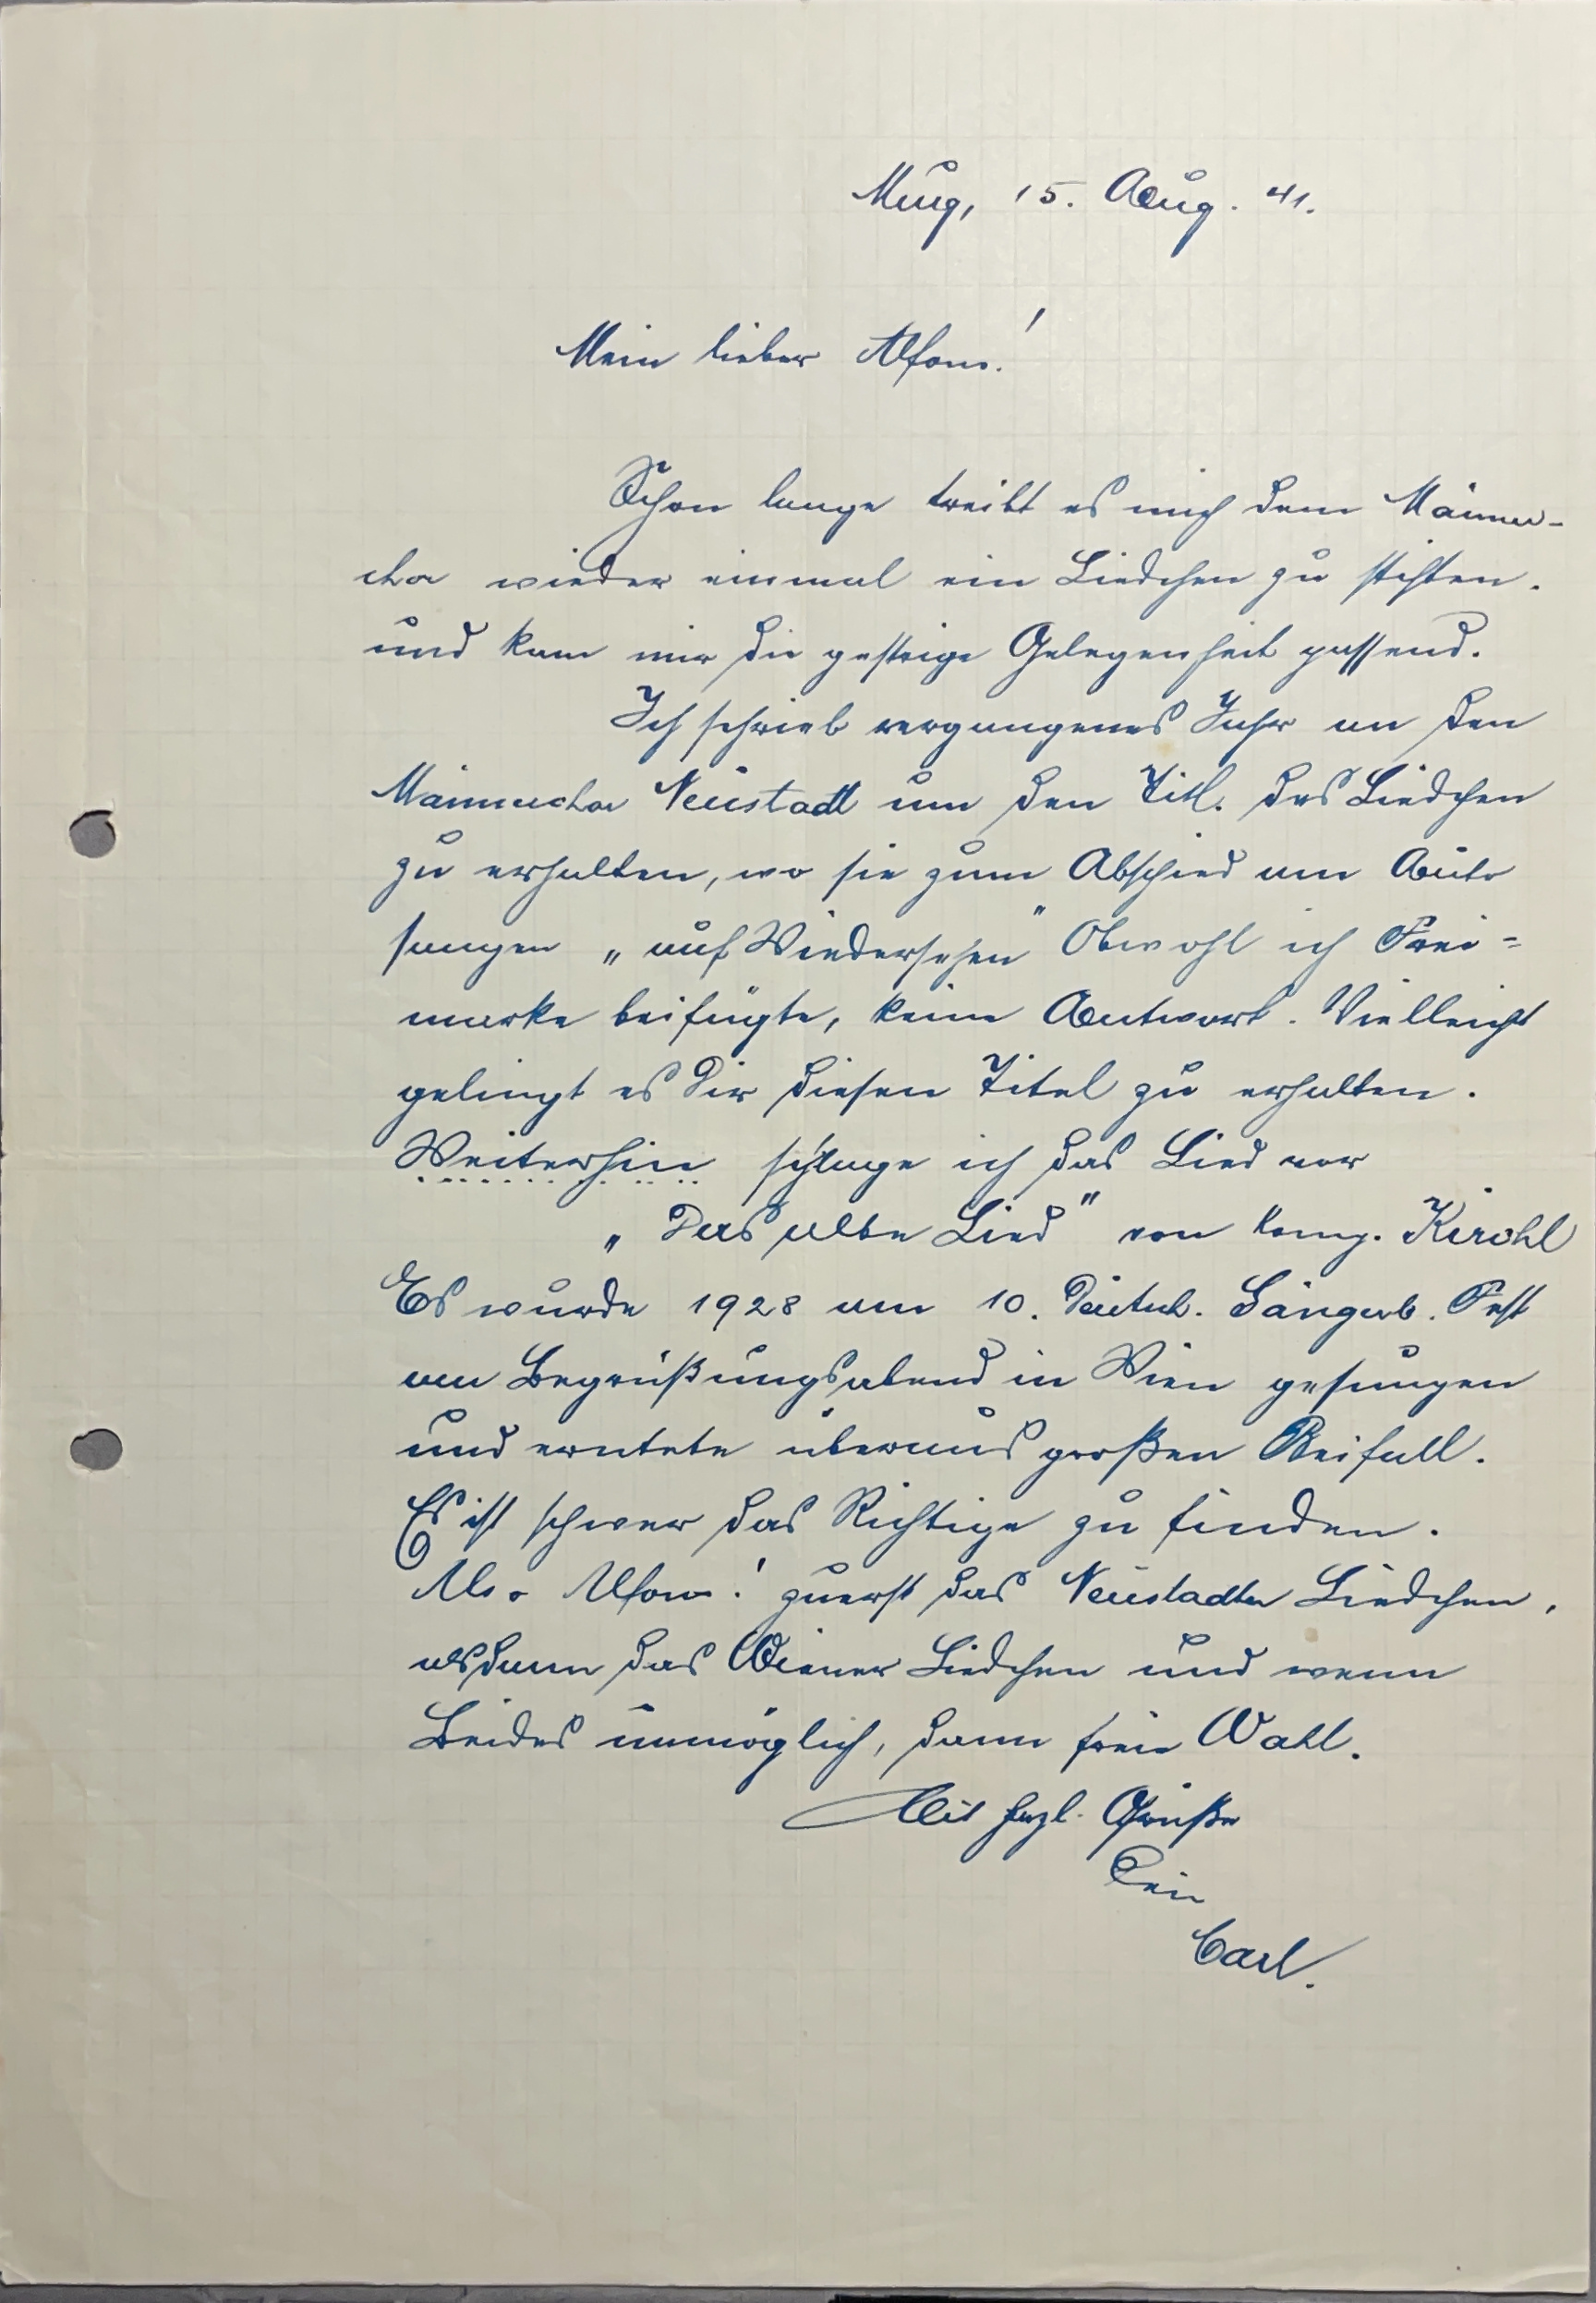
\includegraphics[width=\paperwidth]{./assets/Images/Akte_076_S001.jpg}

  \begin{tcolorbox}[colback=oldLetter, colframe=black, sharp corners, width=\textwidth]
    Murg. 15. Aug 41 \\
    \\
    Mein lieber Alfons! \\
    Sehen lunge Lreitt es mich dem Männer- \\
    chor wieder einmal ein Liedehen zu stehten. \\
    und kam mir die gestege Gelegenheit gussend. \\
    Männechor Venstad um den Title das Liedchen \\
    zu erhalten, wo sie zum Abschied am Aute \\
    sängen „auf Wiederschen Owohl ich Frei! \\
    märke beifügte, keine Aentwarb. Vielleicht \\
    gelingt es Dir diesen Iitel zu erhalten. \\
    Weiterhin sänge ich fal Lied nur \\
    "Bas alte Lied von being. Rerohl \\
    Es wurde 1928 am 10. Dachub. Sängerb. Frst \\
    von Begrüßungsabend in Dien gesungen. \\
    und erntete überaus großen Reifall. \\
    Es ich schwer das Richtige zu finden. \\
    Aler Alfon, werst das Vemsladler Liedchen. \\
    alsdann das Biener Lidchen und wenn \\
    Leides unmöglich, dann freu Nall. \\
    Mit herzl. Grüße \\
    Dein \\
    Carl \\
  \end{tcolorbox}
    ChatGPT produziert daraus:


    \begin{tcolorbox}[colback=oldLetter, colframe=black, sharp corners, width=\textwidth]
    Murg, 15. Aug. 41\\
    \\
Mein lieber Alfons!\\
\\
Schon lange treibt es mich, dem Männerchor wieder einmal ein Liedchen zu stiften, und kam mir die günstige Gelegenheit gelegen.\\
Ich schrieb vergangenes Jahr an den Männerchor Venstad, um den Titel des Liedchens zu erhalten, das sie zum Abschied am Auto sangen: „Auf Wiedersehen, o wohl ich frei!“\\
Ich fügte eine Frankierung bei, erhielt jedoch keine Antwort. Vielleicht gelingt es Dir, diesen Titel zu erhalten.\\
\\
Weiterhin sang ich das Lied nur „Das alte Lied von Wien“. Obwohl es am 10. Dezember 1928 beim Sängerbund-Fest von Begrüßungsabend in Wien gesungen wurde und überaus großen Beifall erntete, ist es schwer, das Richtige zu finden.\\

Aber Alfons, zuerst das Venstadler Liedchen, dann das Wiener Liedchen und wenn beides unmöglich, dann Fröhlichsein.\\

Mit herzlichen Grüßen\\
Dein\\
Carl\\
\end{tcolorbox}

Durch CHatGPT verliert der Text zwar seine ursprüngliche Formatierung und Zeilenumbrüche, aber wird nun nahezu fehlerfrei lesbar. Nur das "Venstadler Liedchen" ist eigendlich eines aus "Neustadt". Eine anschliessende menschliche Korrektur ermöglicht also den Abgeleich mit dem nun lesbaren Text, und die Korrektur der Transkribtion.

Korrigiert und getagt lautet der Brief nun:
\begin{tcolorbox}[colback=oldLetter, colframe=black, sharp corners, width=\textwidth]
  \textbf{\colorbox{place}{\texttt{Murg}}}.  \textbf{\colorbox{date}{\texttt{15. Aug 41}}} \\
\\
Mein lieber  \textbf{\colorbox{person}{\texttt{Alfons}}}!\\
Seit langem treibt es mich dem  \textbf{\colorbox{organization}{\texttt{Männer-}}}\\
\textbf{\colorbox{organization}{\texttt{chor}}} wieder einmal ein Liedchen zu stiften.\\
und kam mir die günstige Gelegenheit passend.\\
Ich schrieb vergangenes Jahhr an den\\
Männechor Vorstand um den Titel das Liedchen\\
zu erhalten, wo sie zum Abschied am Auto \\
sangen "auf Wiederschen" Obwohl ich  \textbf{\colorbox{unclear}{\texttt{Frank-}}}\\
marke beifügte, keine Antwort. Vielleicht\\
gelingt es Dir diesen Titel zu erhalten.\\
Weiterhin sänge ich das Lied nur\\
"Das alte Lied" von  \textbf{\colorbox{abbrev}{\texttt{Komp.}}}\textbf{\colorbox{person}{\texttt{ Kirchl}}}\\
Es wurde \textbf{\colorbox{date}{\texttt{1928}}} am \textbf{\colorbox{eventTag}{\texttt{10. Deutsch. Sängerb. Fest}}}\\
am Begrüßungsabend in \textbf{\colorbox{place}{\texttt{Wien}}} gesungen.\\
und erntete überaus großen Beifall.\\
Es ich schwer das Richtige zu finden.\\
Also \textbf{\colorbox{person}{\texttt{Alfons}}}! zuerst das \textbf{\colorbox{place}{\texttt{Neustadter}}} Liedchen.\\
alsdann das \textbf{\colorbox{place}{\texttt{Wiener}}} Liedchen und wenn\\
Beides unmöglich, dann freie Wahl.\\
Mit herzl. Grüßen \\
Dein\\
\textbf{\colorbox{person}{\texttt{Carl}}}\\
\end{tcolorbox}



      \subsection{Wechsel von Linked Open Data (LOD zu Nodegoat)}
        \subsubsection{Definition und Nutzen von LOD}
        \subsubsection{Aufbau der LOD Ontologie}
        \subsubsection{Gründe für den Wechsel zu Nodegoat}
        \subsubsection{Nodegoat Modelierung}


  \subsection{Netzwerkanalyse als Methode}
        \subsubsection{Theoretischer Hintergrund der Netzwerkanalyse}
        \subsubsection{Ziele der Netzwerkanalyse im Kontext der Quellen}
        \subsubsection{Technische Umsetzung (Tools, Datenbankstruktur)}

\subsection{Normalisierung der Dateien --- von PDF zu JPEG}
\begin{minted}[
frame=lines,
framesep=2mm,
baselinestretch=1.2,
bgcolor=LightGray,
fontsize=\footnotesize,
linenos,
breaklines=true,   % Automatischer Zeilenumbruch
breakanywhere=true % Minted darf überall umbrechen (optional)
]{python}
import os
import fitz  # PyMuPDF

def convert_pdf_to_jpg(src_folder, dest_folder):
    # Überprüfen, ob der Zielordner existiert, und ihn ggf. erstellen
    if not os.path.exists(dest_folder):
        os.makedirs(dest_folder)

    # Durchgehen durch alle Dateien im Quellordner
    for root, dirs, files in os.walk(src_folder):
        for file in files:
            # Überprüfen, ob die Datei eine PDF-Datei ist
            if file.lower().endswith(".pdf"):
                # Vollständigen Pfad zur PDF-Datei erstellen
                pdf_path = os.path.join(root, file)
                # PDF-Datei öffnen
                doc = fitz.open(pdf_path)
                # Durch alle Seiten der PDF-Datei gehen
                for page_num in range(len(doc)):
                    page = doc[page_num]
                    # Seite in ein PixMap-Objekt umwandeln (für die Konvertierung in JPG)
                    pix = page.get_pixmap()
                    # Dateinamen ohne Dateiendung extrahieren
                    filename_without_extension = os.path.splitext(file)[0]
                    # Ausgabedateinamen erstellen mit führenden Nullen für die 
                    # Seitennummer
                    output_filename = f"{filename_without_extension}_S{page_num + 1:03d}.jpg"


                    # Vollständigen Pfad zur Ausgabedatei erstellen
                    output_path = os.path.join(dest_folder, output_filename)
                    # Bild speichern
                    pix.save(output_path)
                # PDF-Datei schließen
                doc.close()
                
                # Erfolgsmeldung ausgeben
                print(f"{file} wurde erfolgreich umgewandelt und gespeichert
                in {dest_folder}")

# Pfade zu den Ordnern mit den PDF-Dateien (Quelle) und den JPG-Dateien (Ziel)
src_folder = r"/Users/svenburkhardt/Documents/D_Murger_Männer_Chor_Forschung/Scan_Männerchor/Männerchor_Akten_1925–1945/Scan_Männerchor_PDF"
dest_folder = r"/Users/svenburkhardt/Documents/D_Murger_Männer_Chor_Forschung/Masterarbeit/JPEG_Akten_Scans"


# Funktion aufrufen, um die Konvertierung durchzuführen
convert_pdf_to_jpg(src_folder, dest_folder)

\end{minted}
\newpage
%--------------------------------------------------------------------------------------%
%--------------------------------------------------------------------------------------%
%------------------------          Aufbau der Datenbank        ----------------------------%
%--------------------------------------------------------------------------------------%
%--------------------------------------------------------------------------------------%

     \section{Aufbau der Datenbank}
    \subsection{Konzeption der Datenmodelieung}
      \subsubsection{Eigene Ontologie im Vergleich zu bestehenden Standards}
      \subsubsection{Verknüpfung von Personen, Orten und Ereignissen}
    
    \subsection{Implementierung der Datenbank}
      \subsubsection{Datenbankdesign}
      \subsubsection{Herausforderungen bei der Datenaufnahme}
      \subsubsection{Verknüpfung mit externen Quellen (z.B. Wikidata)}

    \newpage
%--------------------------------------------------------------------------------------%
%--------------------------------------------------------------------------------------%
%------------------------          Analyse der Netzwerke         ----------------------------%
%--------------------------------------------------------------------------------------%
%--------------------------------------------------------------------------------------%
\section{Analyse der Netzwerke}
  \subsection{Soziale Netzwerke des Vereinslebens}
    \subsubsection{Verbindungen zwischen Mitgliedern}
    \subsubsection{ Kooperationen mit anderen Vereinen}
\subsection{ Politische Netzwerke und deren Veränderungen}
    \subsubsection{Einfluss der NS-Diktatur auf die Netzwerke}
    \subsubsection{Feldpostkarten als Quelle für militärische Netzwerke}
    
 \subsection{ Geografische Ausdehnung der Netzwerke}
  \subsubsection{Einsatzorte der Chormitglieder während des Krieges}
  \subsubsection{ Lokale und überregionale Verbindungen}
  \newpage
%--------------------------------------------------------------------------------------%
%--------------------------------------------------------------------------------------%
%------------------------          Diskussion der Erebnisse         ----------------------------%
%--------------------------------------------------------------------------------------%
%--------------------------------------------------------------------------------------%
\section{Diskussion der Ergebnisse}
  \subsection{Sichtbarmachung der Netzwerke durch Nodegoat und Netzwerkanalyse}
  \subsection{Gibt es Veränderungen der Netzwerke im historischen Kontext?}
  \newpage
%--------------------------------------------------------------------------------------%
%--------------------------------------------------------------------------------------%
%------------------------          Fazit und Ausblick        ----------------------------%
%--------------------------------------------------------------------------------------%
%--------------------------------------------------------------------------------------%
\section{Fazit und Ausblick}
\subsection{Zusammenfassung der zentralen Erkenntnisse}
\subsection{Methodische Herausforderungen und Lösungen}
\subsection{Ausblick auf zukünftige Forschung und mögliche Erweiterungen der Datenbank}
\newpage
%--------------------------------------------------------------------------------------%
%--------------------------------------------------------------------------------------%
%------------------------           Bibliographie      --------------------------------%
%--------------------------------------------------------------------------------------%
%--------------------------------------------------------------------------------------%
\section{Bibliographie}
\printbibliography[
heading=bibintoc,
title={References} % title of the 'references' section, change this if necessary
]

\end{document}
